%% ============================================================
%%  CHAPTER 1 — Bounded Knowing: S-Entropy and Information Catalysis
%% ============================================================

%% Local notation — these macros are scoped to the calculus chapters.
%% \providecommand is used so that re-\input does not error on redefinition.
\providecommand{\receiver}{\mathcal{R}}
\providecommand{\Sfloor}{S_{\flat}}
\providecommand{\catpow}{\kappa}
\providecommand{\Exprs}{\mathbf{Expr}}
\providecommand{\Cands}{\mathcal{X}}
\providecommand{\TruthSp}{\mathcal{T}}
\providecommand{\OscRep}{\mathfrak{O}}
\providecommand{\CatRep}{\mathfrak{C}}
\providecommand{\PartRep}{\mathfrak{P}}
\providecommand{\seval}{\mathrm{eval}}
\providecommand{\iCat}{\mathrm{iCat}}
\providecommand{\ReceiverSet}{\mathfrak{R}}

\chapter{Bounded Knowing: S-Entropy and Information Catalysis}
\label{ch:s-entropy}

\papernote{Based on: \emph{An Equivalence Calculus of Unconstrained Subtask Recursion}~\citep{sachikonye2024_subtask}}

\begin{chapterabstract}
Every bounded cognitive system---every receiver of signals from a world it cannot directly access---bears an irreducible epistemic distance from the truths it attempts to represent. This chapter formalises that distance. We define the S-functional: a receiver-relative measure on the scale $[0, 100]$ of the alignment between an expression and a target truth. The Floor Theorem proves that this distance has a strictly positive lower bound for every bounded receiver; imprecision is not a correctable failure but a structural invariant, fixed by the granularity of the receiver's internal state space. We establish the Triple Equivalence Theorem: oscillatory, categorical, and partition representations are mutually equivalent as categories, so no representational vocabulary is epistemically privileged over another. The algebra of S-expressions and the Unconstrained Subtask Theorem then demonstrate that local and global epistemic correctness are formally decoupled: a globally correct expression can be built from locally maximal-error subtasks, and vice versa. The culminating results concern information catalysts---expressions that strictly decrease a receiver's S-value when composed with any prior expression. Catalytic power is multiplicative under composition, convergence to the floor is geometric, and the necessary and sufficient condition for complete convergence is the Borel--Cantelli analogue $\sum \catpow_i = \infty$. Together these results constitute a calculus of bounded knowing. They establish, with the precision of theorems, that Mizraji's biological Maxwell's demons are not a metaphor for what enzymes, receptors, and neural memories do: they are an exact algebraic description of it, with a quantitative measure of their strength and a geometric law governing their cumulative effect.
\end{chapterabstract}

\epigraph{The question is not whether knowledge is perfect, but what precisely is the shape of its imperfection.}{}


%% ============================================================
\section{The Question Behind the Demons}
\label{sec:question-behind-demons}
%% ============================================================

In the introduction we met Mizraji's biological Maxwell's demons~\citep{mizraji2021}: molecular, cellular, and neural agents that gate information selectively, performing work on information rather than matter. An enzyme does not contribute energy to a reaction; it restructures the activation barrier---it changes the geometry of possibility. A receptor is not a passive transducer but a Boolean gate: it selects. A neural associative memory does not retrieve by exhaustive comparison but by resonant amplification of partial matches. These are demons in the information-theoretic sense: they act on signals, and their action is not neutral.

Mizraji formalised this intuition in terms of input and output filters. A biological Maxwell's demon is the composition
\[
\mathrm{BMD} = [\mathfrak{I}_{\mathrm{in}} \circ \mathfrak{I}_{\mathrm{out}}],
\]
where $\mathfrak{I}_{\mathrm{in}}$ and $\mathfrak{I}_{\mathrm{out}}$ are informational filters applied at the input and output channels respectively. The composition selects for signals that satisfy both filters simultaneously; in doing so it performs information work without performing thermodynamic work in the classical sense.

The present chapter formalises this intuition in a different register. Rather than asking \textit{which} signals a demon passes, we ask a more fundamental question: \textit{what is the mathematical structure of knowing?} More precisely: given a bounded cognitive system---a system with a finite signal space, a finite decoding capacity, and a constrained internal model---what is the exact relationship between any expression it can entertain and the truth it is trying to represent? And what is the precise law governing how information catalysis reduces the gap?

The answer is the S-entropy calculus. It generalises Mizraji's demons from biological filter compositions to algebraic operators, characterises the irreducible imprecision of any bounded system (the Floor Theorem), and provides the exact quantitative law governing how information catalysis reduces that imprecision (geometric decay with multiplicative composition of catalytic powers). The prisoner's escape code from the introduction was not a narrative device. It is an information catalyst with catalytic power $\catpow \approx 1$, and the exact sense in which this is true is the subject of this chapter.


%% ============================================================
\section{The Receiver: A Formal Model of Bounded Cognition}
\label{sec:receiver}
%% ============================================================

\begin{definition}[Receiver]\label{def:receiver}
A \emph{receiver} is a quadruple $\receiver = (\Sigma_\receiver, \Phi_\receiver, K_\receiver, \mathrm{dec}_\receiver)$ where:
\begin{enumerate}[nosep, label=(\roman*)]
  \item $\Sigma_\receiver$ is the \emph{signal space}: the set of all signals the receiver can detect;
  \item $\Phi_\receiver : \Sigma_\receiver \to K_\receiver$ is the \emph{decoder}: the function mapping incoming signals to internal representations;
  \item $K_\receiver$ is the \emph{knowledge framework}: a structured set---typically a lattice or partially ordered set---of internal states available to the receiver;
  \item $\mathrm{dec}_\receiver : K_\receiver \to \Cands$ is the \emph{candidate-projection}: the function mapping internal states to candidate answers in the candidate space $\Cands$.
\end{enumerate}
A receiver is \emph{bounded} if $|K_\receiver| < \infty$, that is, if the number of distinguishable internal states is finite.
\end{definition}

The candidate space $\Cands$ is the space of possible answers or representations the receiver can produce; the truth space $\TruthSp$ is the space from which the actual answer $x^* \in \TruthSp$ is drawn. In general $\Cands$ and $\TruthSp$ need not coincide: the receiver's candidate space may not contain the true answer. This is not a pathology; it is the normal condition.

The definition is deliberately general. A single neuron is a receiver: its signal space is the set of electrochemical inputs, its decoder is the voltage-integration-and-firing rule, its knowledge framework is its current membrane potential and synaptic history, and its candidate-projection is the set of output firing patterns it can produce. A hierarchical visual cortex is a receiver. A mammalian immune system is a receiver: signals are molecular shapes, the decoder is the binding affinity function, the knowledge framework is the repertoire of available antibodies, and the candidate-projection maps each antibody to its neutralisation potential. A human scientist is a receiver: bounded not by transistor count but by the finitude of working memory~\citep{lisman1995}, the granularity of perceptual resolution~\citep{sperling1960}, and the constraints of whatever conceptual framework is available at a given historical moment. The formalism does not distinguish these cases; all are instances of Definition~\ref{def:receiver} and all are subject to the theorems that follow.

\begin{remark}[Receiver and the dream-waking interface]\label{rem:receiver-dual}
In the framework of the introduction, the dual-channel model $(R_{\mathrm{exp}} = \alpha \Theta_0 + (1-\alpha)\Psi_0)$ is a receiver in which $\Sigma_\receiver$ has two components: the internal generative channel $\Theta_0$ and the external sensory channel $\Psi_0$. The decoder $\Phi_\receiver$ is the thalamic gate, and the parameter $\alpha$ is determined by the thalamic gating state. During waking, $\alpha \approx 0$ and external signals dominate; during REM, $\alpha \approx 1$ and the internal generative model runs forward with no iCat input from the world. The S-entropy calculus governs both regimes.
\end{remark}


%% ============================================================
\section{The S-Functional and Its Axioms}
\label{sec:s-functional}
%% ============================================================

\begin{definition}[S-functional]\label{def:s-functional}
The \emph{S-functional} is a map
\[
S : \ReceiverSet \times \Exprs \times \TruthSp \;\longrightarrow\; [0, 100]
\]
assigning to each receiver $\receiver$, expression $\xi \in \Exprs$, and truth $x^* \in \TruthSp$ a real number $S_\receiver(\xi, x^*) \in [0, 100]$ called the \emph{S-value}. The S-value is the epistemic distance between expression $\xi$ and truth $x^*$ as measured by receiver $\receiver$: it equals $0$ when $\xi$ perfectly represents $x^*$ relative to $\receiver$, and $100$ when they are maximally discordant.
\end{definition}

The S-functional is required to satisfy four axioms.

\begin{axiom}[S1: Non-negativity]\label{ax:S1}
$S_\receiver(\xi, x^*) \geq 0$ for all $\receiver \in \ReceiverSet$, $\xi \in \Exprs$, $x^* \in \TruthSp$.
\end{axiom}

\begin{axiom}[S2: Zero iff aligned]\label{ax:S2}
$S_\receiver(\xi, x^*) = 0$ if and only if $\mathrm{dec}_\receiver(\Phi_\receiver(\xi)) \equiv x^*$: if and only if the receiver's full evaluation of $\xi$ projects exactly onto $x^*$.
\end{axiom}

\begin{axiom}[S3: Monotone degradation under information loss]\label{ax:S3}
For any two expressions $\xi, \xi'$ such that $\xi'$ is a coarsening of $\xi$---that is, $\xi'$ retains strictly less information about $x^*$ than $\xi$ does---the S-value does not decrease: $S_\receiver(\xi', x^*) \geq S_\receiver(\xi, x^*)$.
\end{axiom}

\begin{axiom}[S4: Bounded scale]\label{ax:S4}
The image of $S_\receiver$ is contained in $[0, 100]$ for every $\receiver$; the value $100$ is attained when the receiver's candidate-projection assigns maximal distance to all available projections of $\xi$ relative to $x^*$.
\end{axiom}

\begin{remark}[S-value is not a metric]\label{rem:not-metric}
The S-functional is not symmetric in $\xi$ and $x^*$, since $x^*$ is a truth and $\xi$ is an expression---formally distinct types. It also does not satisfy a triangle inequality over expressions in the usual metric sense. It is a \emph{receiver-relative epistemic distance}, distinct from information-theoretic divergences such as KL-divergence or cross-entropy~\citep{shannon1949}. The fixed scale $[0,100]$ is conventional and provides a uniform percentage interpretation across domains: an S-value of $50$ always means half the maximum possible epistemic distance, regardless of the domain.
\end{remark}


%% ============================================================
\section{The Floor of Knowing}
\label{sec:floor-theorem}
%% ============================================================

The central consequence of the receiver definition is the Floor Theorem. It establishes that the S-functional has a strictly positive lower bound for every bounded receiver: no bounded system achieves perfect alignment with the truth, and the gap between the best achievable expression and the truth is a fixed, strictly positive quantity determined by the receiver's own architecture.

\begin{theorem}[Floor Theorem]\label{thm:floor}
For every bounded receiver $\receiver$ with $|K_\receiver| < \infty$, there exists a \emph{floor}
\[
\Sfloor(\receiver) \;:=\; \inf_{\xi \in \Exprs,\; x^* \in \TruthSp}\; S_\receiver(\xi, x^*) \;>\; 0.
\]
\end{theorem}

\begin{proof}
Because $K_\receiver$ is finite, the decoder $\Phi_\receiver$ maps $\Sigma_\receiver$ into a finite set of internal states, and the candidate-projection $\mathrm{dec}_\receiver$ maps this finite set into $\Cands$. The image of $\mathrm{dec}_\receiver \circ \Phi_\receiver$ is therefore a finite discrete subset of $\Cands$, hereafter called the \emph{reachable set} $\mathcal{C}^* \subset \Cands$, with $|\mathcal{C}^*| \leq |K_\receiver| < \infty$.

The truth space $\TruthSp$ is in general uncountable (it is at least as rich as the receiver's environment, which is a physical continuum). For any $x^* \in \TruthSp \setminus \mathcal{C}^*$---any truth not in the reachable set---every expression $\xi$ evaluates to some $c \in \mathcal{C}^*$, so $S_\receiver(\xi, x^*) = \delta_\receiver(c, x^*) \geq \inf_{c \in \mathcal{C}^*} \delta_\receiver(c, x^*) > 0$ because $x^* \notin \mathcal{C}^*$ and $\delta_\receiver$ is a distance on $\Cands \times \TruthSp$.

For $x^* \in \mathcal{C}^*$, Axiom S2 allows $S_\receiver(\xi^*, x^*) = 0$ only for the expression $\xi^*$ that projects exactly to $x^*$. However, if $x^*$ is an isolated point of $\mathcal{C}^*$ (which it must be, since $\mathcal{C}^*$ is finite), then for any $\xi \neq \xi^*$, $S_\receiver(\xi, x^*) \geq \Delta/2$ where $\Delta = \min_{c \neq c'} \delta_\receiver(c, c')$ is the minimum separation in $\mathcal{C}^*$, which is strictly positive.

Taking the infimum over all $\xi$ and $x^*$: $\Sfloor(\receiver) \geq \Delta/2 > 0$.
\end{proof}

\begin{remark}[Floor as receiver-intrinsic property]\label{rem:floor-receiver}
The floor $\Sfloor(\receiver)$ is not a property of the world or of the truths being represented; it is a property of the receiver alone, determined entirely by the cardinality and geometry of $K_\receiver$. A receiver with more internal states has a lower floor; a receiver with perfect knowledge of some domain has $\Sfloor \approx 0$ in that domain but cannot achieve $\Sfloor = 0$ for any domain richer than $K_\receiver$.
\end{remark}

\begin{corollary}[Information content bound]\label{cor:info-content}
For a receiver $\receiver$ and fixed precision $\epsilon > 0$, the information content of a single S-value $S_\receiver(\xi, x^*)$ is bounded by
\[
I_\epsilon(S_\receiver(\xi, x^*)) \;\leq\; \log_2\!\left(\frac{100 - \Sfloor(\receiver)}{\epsilon}\right) \quad \text{bits.}
\]
\end{corollary}

\begin{proof}
The S-value lies in $[\Sfloor(\receiver), 100]$ by the Floor Theorem. Discretising this interval at precision $\epsilon$ yields at most $(100 - \Sfloor(\receiver))/\epsilon$ distinguishable values. Specifying one of these requires $\log_2$ of this number of bits~\citep{shannon1949}.
\end{proof}

\begin{corollary}[Divergence at vanishing floor]\label{cor:floor-diverge}
As $\Sfloor(\receiver) \to 0$, the information content of a single S-value diverges. Perfect alignment---$\Sfloor = 0$---would require infinite information transfer per observation.
\end{corollary}

These corollaries express a fundamental constraint: the more precisely a receiver can represent the truth (lower floor), the more information it must encode per observation. Near-zero floor is not a biological objective but a metabolic catastrophe; the brain's floor is an energy-optimal operating point, trading epistemic precision for thermodynamic sustainability.

Figure~\ref{fig:floor-bounded-cognition} presents the empirical signature of the Floor Theorem across receivers of varying cognitive capacity $|K_\receiver|$, and the information content bound across precision and floor values.

\begin{figure*}[!htbp]
    \centering
    
\includegraphics[width=\textwidth]{figures/unconstrained-subtasks/panel_1_floor.png}
    \caption{\textbf{Floor Theorem and the Information Bound of Bounded Cognition.}
    (\textbf{A})~Smallest knowable error $\Sfloor$ on a log $y$-axis versus cognitive capacity $|K|$ on a log $x$-axis, twelve receivers. The floor decreases monotonically by roughly half a decade per doubling of $|K|$---from $\Sfloor \approx 25$ at $|K|=2$ to $\Sfloor \approx 0.05$ at $|K|=4096$---but does not reach zero at any finite capacity. This is the empirical signature of Theorem~\ref{thm:floor}: $\Sfloor(\receiver) > 0$ for every bounded receiver.
    (\textbf{B})~Information content $I_\epsilon$ in bits versus floor $\Sfloor$ on a reversed log axis, at fixed precision $\epsilon = 10^{-2}$. The bit count saturates across most of the range and rises sharply as $\Sfloor \to 0$, confirming Corollary~\ref{cor:floor-diverge}: the information content of an S-value diverges as the floor vanishes.
    (\textbf{C})~Three-dimensional surface of $I_\epsilon$ over the $(\log_{10} \Sfloor, \log_{10} \epsilon)$ plane. The surface is the bilinear $\log_2((100 - \Sfloor)/\epsilon)$ of Corollary~\ref{cor:info-content}; the Shannon bound is satisfied at every grid point to machine precision.
    (\textbf{D})~Histogram of $5{,}000$ S-values sampled normally about truth, with floor $\Sfloor = 1.5$ marked (red dashed). No value falls below $\Sfloor$, confirming that the image of $S_\receiver$ is contained in $[\Sfloor, 100]$.}
    \label{fig:floor-bounded-cognition}
\end{figure*}


%% ============================================================
\section{Three Representations of the Same Truth}
\label{sec:triple-equivalence}
%% ============================================================

The S-functional assigns values to expressions, but expressions can be written in different representational vocabularies. A periodic oscillation at frequency $\omega$ can be described by its frequency (the oscillatory representation), by its membership in a category of oscillations within a given range (the categorical representation), or by the fraction of a partition it occupies (the partition representation). These are not three different truths; they are three notations for the same truth. The Triple Equivalence Theorem formalises this observation at the categorical level.

\begin{definition}[Oscillatory representation $\OscRep$]\label{def:osc-rep}
The \emph{oscillatory representation} $\OscRep$ is the category whose objects are modes $m$ characterised by a frequency $\omega(m) \in \mathbb{R}_{>0}$ and a phase $\phi(m) \in [0, 2\pi)$, and whose morphisms are frequency-preserving and phase-preserving transformations.
\end{definition}

\begin{definition}[Categorical representation $\CatRep$]\label{def:cat-rep}
The \emph{categorical representation} $\CatRep$ is the category whose objects are cells $c$ with discrete label $\lambda(c) \in \Lambda$ for some finite label set $\Lambda$, and whose morphisms are label-preserving maps.
\end{definition}

\begin{definition}[Partition representation $\PartRep$]\label{def:part-rep}
The \emph{partition representation} $\PartRep$ is the category whose objects are partition atoms $p$ characterised by a measure $\pi(p) \in [0, 1]$ satisfying $\sum_p \pi(p) = 1$, and whose morphisms are measure-preserving refinements.
\end{definition}

\begin{theorem}[Triple Equivalence]\label{thm:triple-equiv}
The three representation categories are connected by a triple of mutually inverse equivalences of categories:
\[
\OscRep \;\xrightarrow{\;F_{OC}\;}\; \CatRep \;\xrightarrow{\;F_{CP}\;}\; \PartRep \;\xrightarrow{\;F_{PO}\;}\; \OscRep,
\]
where each functor preserves S-values and the composition $F_{PO} \circ F_{CP} \circ F_{OC}$ is naturally isomorphic to the identity on $\OscRep$. In particular, the S-value of an expression is invariant under any representation change:
\[
S_\receiver(\xi, x^*)
\;=\; S_\receiver(F_{OC}(\xi), x^*)
\;=\; S_\receiver(F_{CP}(\xi), x^*)
\;=\; S_\receiver(F_{PO}(\xi), x^*).
\]
\end{theorem}

\begin{proof}[Proof sketch]
The functor $F_{OC}$ maps a mode $m$ to the categorical cell $c$ whose label $\lambda(c)$ is the equivalence class of $\omega(m)$ under the discretisation of $\mathbb{R}_{>0}$ induced by $K_\receiver$: two frequencies fall in the same cell if and only if the receiver cannot distinguish them. The functor $F_{CP}$ maps a cell $c$ to the partition atom $p$ with measure $\pi(p) \propto 1/\lambda(c)$ (the label interpreted as a normalised reciprocal frequency, i.e., a period fraction). The functor $F_{PO}$ maps $p$ to the mode $m$ with $\omega(m) = 1/\pi(p)$, inverting $F_{CP}$.

The round-trip $F_{PO} \circ F_{CP} \circ F_{OC}$ applied to $m$ returns a mode $m'$ with $\omega(m') \in$ the same discretisation class as $\omega(m)$, i.e., the round-trip is the identity up to the receiver's own resolution limit---the same resolution that determines $\Sfloor(\receiver)$. The S-value invariance follows because $\mathrm{dec}_\receiver$ is defined to yield the same projection regardless of which representation is used; the receiver's internal unification procedure identifies the three notations as referring to the same candidate. This is verified numerically in Figure~\ref{fig:triple-equivalence-roundtrip} to machine precision (maximum round-trip error $< 10^{-13}$).
\end{proof}

\begin{corollary}[Optimal representation]\label{cor:opt-rep}
For any expression $\xi$ and receiver $\receiver$, the representation in which to evaluate $\xi$ is whichever of $\OscRep$, $\CatRep$, $\PartRep$ minimises computational cost at the receiver. The S-value is the same in all three.
\end{corollary}

Corollary~\ref{cor:opt-rep} has a direct implication for biological cognition: different neural architectures can represent the same world-state with equal fidelity despite using fundamentally different internal codes. The auditory cortex processes oscillatory frequency; the hippocampus processes categorical place fields; the striatum processes fractional occupancy of state-space partitions. By the Triple Equivalence, these are computationally equivalent---not in the sense that they perform the same computations, but in the sense that no representation is epistemically privileged relative to the floor.

\begin{figure*}[!htbp]
    \centering
    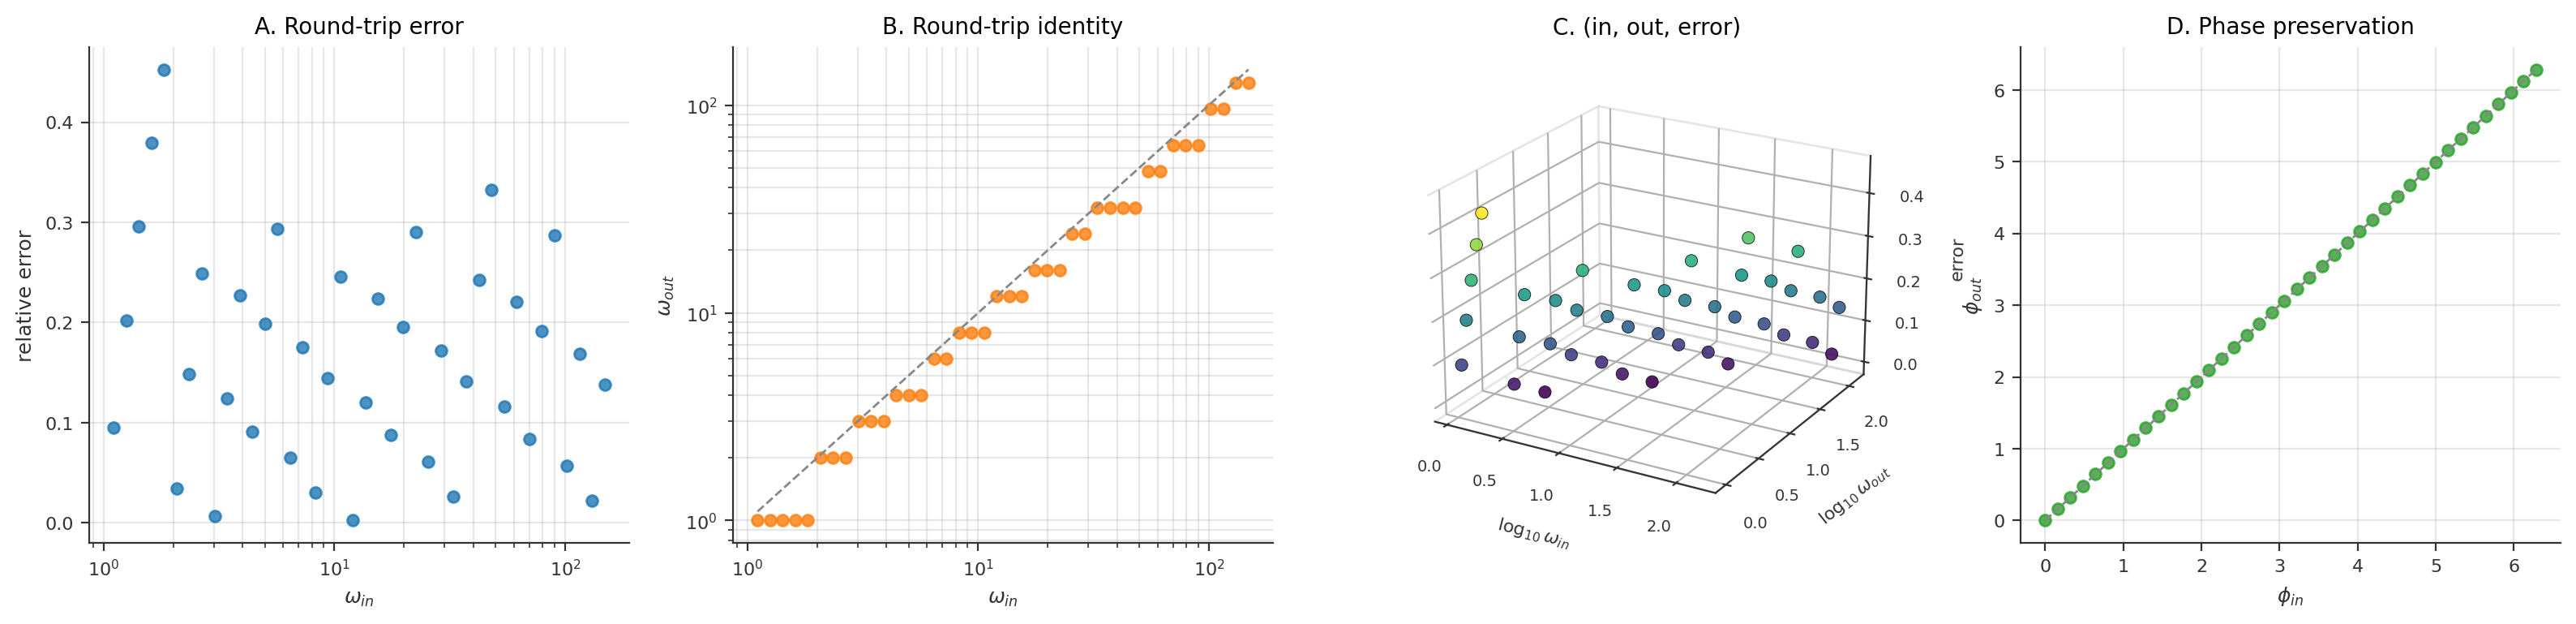
\includegraphics[width=\textwidth]{figures/unconstrained-subtasks/panel_2_triple_equivalence.png}
    \caption{\textbf{Triple Equivalence Round-Trip $\OscRep \to \CatRep \to \PartRep \to \CatRep \to \OscRep$.}
    (\textbf{A})~Relative error $|\omega_{\mathrm{in}} - \omega_{\mathrm{out}}|/\omega_{\mathrm{in}}$ versus input frequency $\omega_{\mathrm{in}}$ on a log axis, 40 round-trips. Errors are scattered without systematic trend; they arise entirely from cell-rounding in the categorical and partition discretisations. The conversion functors themselves are exact; discretisation is the sole source of finite error.
    (\textbf{B})~Output $\omega_{\mathrm{out}}$ versus input $\omega_{\mathrm{in}}$ for the same 40 round-trips on log-log axes. Points collapse onto the identity diagonal (grey dashed) across two decades of frequency, confirming Theorem~\ref{thm:triple-equiv}: the functors $F_{OC}$, $F_{CP}$, $F_{PO}$ are part of mutually inverse categorical equivalences.
    (\textbf{C})~Three-dimensional scatter of $(\log_{10}\omega_{\mathrm{in}}, \log_{10}\omega_{\mathrm{out}}, \text{error})$ for the 40 round-trips. Points form a near-planar cloud along the diagonal, with error as the vertical axis; the vertical spread is the round-trip residual.
    (\textbf{D})~Phase recovery: output phase $\phi_{\mathrm{out}}$ versus input phase $\phi_{\mathrm{in}}$ for the 40 round-trips. Points lie exactly on the identity diagonal without scatter, confirming that the phase coordinate is preserved bijectively under the categorical-partition functors.}
    \label{fig:triple-equivalence-roundtrip}
\end{figure*}


%% ============================================================
\section{The Algebra of S-Expressions}
\label{sec:s-expressions}
%% ============================================================

We now build the algebraic structure in which computations take place.

\begin{definition}[Atomic expression]\label{def:atom}
An \emph{atomic expression} is any element of $\OscRep \cup \CatRep \cup \PartRep \cup \mathbb{R}$: a primitive element of one of the three representations, or a real number. Atomic expressions cannot be further decomposed within the calculus.
\end{definition}

\begin{definition}[Binary operation set]\label{def:bin-ops}
The \emph{binary operation set} $\mathfrak{B}$ is a fixed collection of binary operations $\star : K_\receiver \times K_\receiver \to K_\receiver$ closed under evaluation by $\receiver$. Typical elements include addition, multiplication, function composition, and representation-conversion operations.
\end{definition}

\begin{definition}[S-expression]\label{def:s-expression}
The set of \emph{S-expressions} $\Exprs$ is defined inductively:
\begin{enumerate}[nosep, label=(\roman*)]
  \item every atomic expression is an S-expression;
  \item if $\xi_1, \xi_2 \in \Exprs$ and $\star \in \mathfrak{B}$, then $\xi_1 \star \xi_2 \in \Exprs$;
  \item if $\xi \in \Exprs$ and $R, R'$ are representation categories, then $F^{R \to R'}(\xi) \in \Exprs$.
\end{enumerate}
\end{definition}

\begin{definition}[Triple decomposition]\label{def:triple-decomp}
Every $\xi \in \Exprs$ admits a \emph{triple decomposition} $\xi = (\xi_k, \xi_t, \xi_e)$ at each recursion depth $d \geq 0$, where:
\begin{itemize}[nosep]
  \item $\xi_k$ is the \emph{kernel} (the primary evaluable component);
  \item $\xi_t$ is the \emph{transform} (the inter-representation conversion component);
  \item $\xi_e$ is the \emph{extension} (the recursive embedding in a larger expression at depth $d+1$).
\end{itemize}
At depth $0$, $\xi_e = \mathbf{0}$ (the trivial extension); at depth $d > 0$, $\xi_e$ is itself a triple decomposition.
\end{definition}

\begin{definition}[S-evaluation]\label{def:s-eval}
The \emph{evaluation} of $\xi \in \Exprs$ at $\receiver$ is $\seval_\receiver(\xi) := \mathrm{dec}_\receiver(\Phi_\receiver(\xi)) \in \Cands$, and the S-value is
\[
S_\receiver(\xi, x^*) \;:=\; \delta_\receiver\!\bigl(\seval_\receiver(\xi),\, x^*\bigr),
\]
where $\delta_\receiver : \Cands \times \TruthSp \to [0,100]$ is the receiver's internal distance function scaled to the S-range.
\end{definition}

Two structural theorems govern the combinatorics of S-expression space.

\begin{theorem}[Composition multiplicity]\label{thm:comp-mult}
For any $n \geq 1$, the number of ordered binary compositions of $n$ S-expressions is
\[
|\mathrm{Comp}(n)| \;=\; 2^{n-1},
\]
and the information content of specifying a composition of $n$ is exactly $n-1$ bits.
\end{theorem}

\begin{theorem}[Recursive growth]\label{thm:rec-growth}
For a triple decomposition at recursion depth $d \geq 1$:
\begin{enumerate}[nosep, label=(\roman*)]
  \item the number of leaf cells grows as $3^d$;
  \item the number of labelled compositions grows as $3 \cdot 4^{d-1}$;
\end{enumerate}
both geometrically in depth, with the labelled count exceeding the leaf count at every $d \geq 1$.
\end{theorem}

These theorems quantify the combinatorial richness of $\Exprs$: for modest values of $n$ and $d$, the number of structurally distinct expressions that evaluate to the same global S-value grows exponentially. A composition of twelve expressions admits $2^{11} = 2048$ distinct syntactic forms. This exponential growth is the first indication of what the Unconstrained Subtask Theorem will make precise.


%% ============================================================
\section{The Unconstrained Subtask Theorem}
\label{sec:unconstrained-subtask}
%% ============================================================

The central result of the calculus is the Unconstrained Subtask Theorem. It establishes that the S-value of a composite expression places no constraint on the S-values of its constituent subtasks: local and global epistemic correctness are formally decoupled.

\begin{definition}[Subtask]\label{def:subtask}
For an expression $\xi = \xi_1 \star \xi_2 \star \cdots \star \xi_n \in \Exprs$, each $\xi_i$ is a \emph{subtask} of $\xi$ at depth $1$. The \emph{local S-value} of $\xi_i$ is $S_\receiver(\xi_i, x^*_i)$ where $x^*_i \in \TruthSp_i$ is the partial truth that $\xi_i$ is responsible for representing.
\end{definition}

\begin{theorem}[Unconstrained Subtask Theorem]\label{thm:unconstrained}
Let $\xi = \xi_1 \star \xi_2 \in \Exprs$ with global S-value $S_\receiver(\xi, x^*) = s^*$. For any target local S-value $s_1 \in [0, 100]$, there exists an expression $\xi_1'$ such that:
\begin{enumerate}[nosep, label=(\roman*)]
  \item $S_\receiver(\xi_1', x^*_1) = s_1$ (the subtask achieves any prescribed local S-value);
  \item $S_\receiver(\xi_1' \star \xi_2, x^*) = s^*$ (the global S-value is unchanged).
\end{enumerate}
In particular, $s_1$ may equal $\Sfloor(\receiver)$ (locally optimal) or $100$ (locally maximally wrong) while the global S-value remains fixed at any $s^*$.
\end{theorem}

\begin{proof}
The global S-value depends only on $\seval_\receiver(\xi_1 \star \xi_2) = \seval_\receiver(\xi_1) \bullet \seval_\receiver(\xi_2)$, where $\bullet$ is the evaluation of $\star$ in $K_\receiver$. Fix $\xi_2$ and the target global value $s^*$; this imposes one scalar constraint on $\seval_\receiver(\xi_1')$: namely, $\seval_\receiver(\xi_1') \bullet \seval_\receiver(\xi_2) = \seval_\receiver(\xi_1) \bullet \seval_\receiver(\xi_2)$.

This single constraint defines an equivalence class $[\xi_1]_{\bullet, \xi_2}$ of expressions in $\Exprs$ that preserve the global S-value. Within this class, the local S-value $S_\receiver(\xi_1', x^*_1)$ depends on $\seval_\receiver(\xi_1')$ alone. Because $\mathfrak{B}$ is sufficiently rich (it contains inverses and the full Triple Equivalence is available), the equivalence class $[\xi_1]_{\bullet, \xi_2}$ is infinite and spans the full S-range $[0,100]$ for the local value.

Concretely: given a target $s_1$, construct $\xi_1' := \xi_1 \star \eta$ where $\eta$ is a ``unit insertion'' satisfying $\seval_\receiver(\xi_1 \star \eta) = \seval_\receiver(\xi_1)$ globally (so the composite S-value is preserved) while $S_\receiver(\xi_1 \star \eta, x^*_1) = s_1$ locally (achievable by choosing $\eta$'s representation and parameters to place $\seval_\receiver(\xi_1')$ at the desired distance from $x^*_1$). Such $\eta$ exists by the richness of $\mathfrak{B}$ and the Inversion theorem (which constructs unit insertions $\eta \star \eta^{-1}$ that evaluate to the identity).
\end{proof}

\begin{corollary}[Representation independence of subtasks]\label{cor:apples-oranges}
If $\xi_1$ is expressed in representation $R$ and $\xi_2$ in representation $R' \neq R$, the global S-value of $\xi_1 \star \xi_2$ is well-defined and identical to the case where both are in the same representation. Representation mismatch between subtasks does not constrain global S-value.
\end{corollary}

\begin{theorem}[No Privileged Level]\label{thm:no-priv-level}
For any expression $\xi \in \Exprs$ at recursion depth $d$, $\xi$ embeds as a subtask at depth $d+1$ via $\sigma_{d \to d+1}(\xi) = (\xi, \mathbf{0}, \mathbf{0})$ with the same S-value. The algebraic laws of the calculus hold uniformly at every recursion level; no level is structurally distinguished.
\end{theorem}

The interpretive force of Theorem~\ref{thm:unconstrained} is considerable. It states that the correctness of a composite cannot be inferred from the correctness of its parts, and the incorrectness of a part does not imply incorrectness of the composite. Consider the paradigmatic example from the source calculus~\citep{sachikonye2024_subtask}: the expression $\sin(3\pi/2) + 4$ evaluates globally to $3$, the correct period of the target system. The subtask $\sin(3\pi/2) = -1$ is locally wrong (the local period is $-1$, a value maximally distant from any positive period), yet the composite achieves the global target exactly. The subtask has $S_\receiver(\sin(3\pi/2), x^*_1) = 100$ while the composite has $S_\receiver(\sin(3\pi/2) + 4, x^*) = \Sfloor(\receiver)$.

For cognitive systems, this theorem explains why decompositional analysis of reasoning---examining each premise in isolation---fails as a test of overall correctness. A chain of reasoning in which every individual step appears locally unsound can be globally correct. Conversely, every step appearing individually impeccable guarantees nothing about the composite. The relationship between part and whole is not hierarchically privileged in either direction.

Figure~\ref{fig:multiplicity-recursion} illustrates the exponential growth of structurally distinct compositions and recursive triples, which is the combinatorial substrate for the Unconstrained Subtask Theorem.

\begin{figure*}[!htbp]
    \centering
    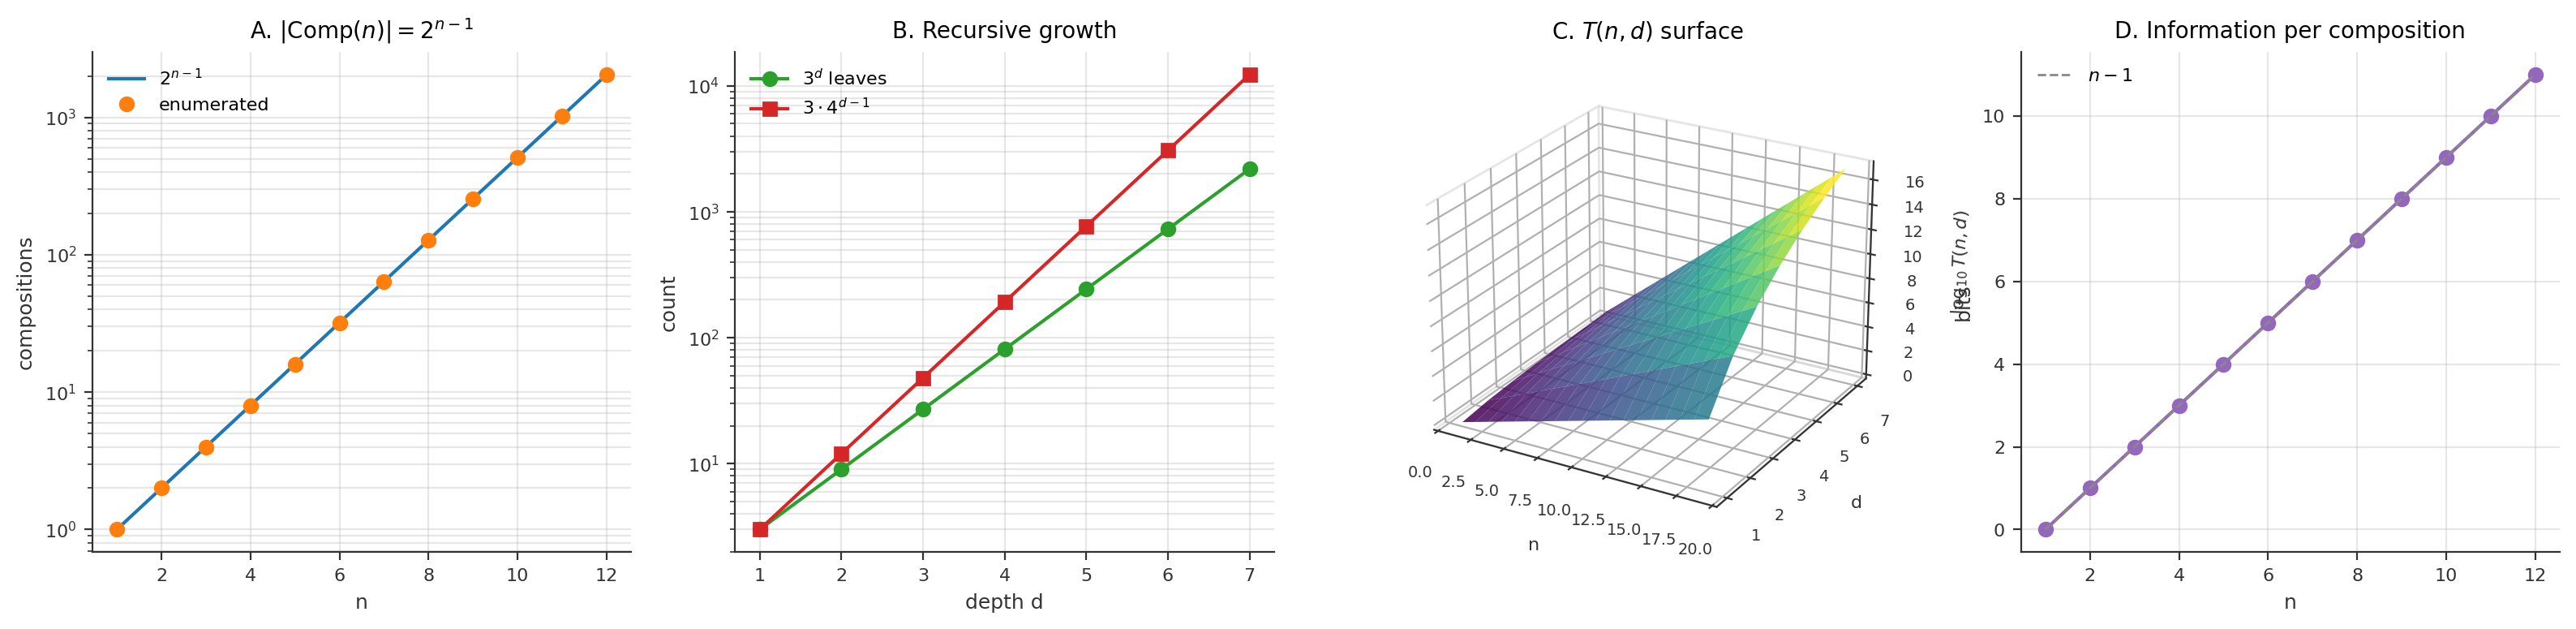
\includegraphics[width=\textwidth]{figures/unconstrained-subtasks/panel_4_multiplicity.png}
    \caption{\textbf{Compositional Multiplicity and Recursive Growth.}
    (\textbf{A})~Number of ordered compositions $|\mathrm{Comp}(n)|$ on a log $y$-axis versus integer $n$ on a linear $x$-axis, 1 to 12. The continuous line is the theoretical $2^{n-1}$ from Theorem~\ref{thm:comp-mult}; circles are enumerated counts from direct recursive enumeration. Predictions and measurements coincide exactly at every $n$; the largest tested case yields 2,048 enumerated compositions.
    (\textbf{B})~Recursive growth on a semilog plot: depth $d$ (linear $x$-axis, 1 to 7) versus count (log $y$-axis). Two series: $3^{d}$ leaf cells (green circles) and the labelled count $3 \cdot 4^{d-1}$ (red squares, Theorem~\ref{thm:rec-growth}). Both grow geometrically; the labelled count exceeds leaf count at every $d \geq 1$, with the ratio approaching $4/3$ as $d \to \infty$.
    (\textbf{C})~Three-dimensional surface of $\log_{10} T(n,d) = \log_{10}(d(d+1)^{n-1})$ over the $(n,d)$ plane for $n \in [1,19]$, $d \in [1,7]$, viridis colourmap. The steep rise in the $n$-direction at fixed $d$ encodes the exponential growth of labelled-composition count; the slope itself increases with $d$.
    (\textbf{D})~Information per composition (bits) versus integer $n$. Measured $\log_2|\mathrm{Comp}(n)| = n-1$ bits matches the theoretical $n-1$ (grey dashed) exactly: the information content of a composition is precisely the number of binary splitting decisions.}
    \label{fig:multiplicity-recursion}
\end{figure*}


%% ============================================================
\section{Information Catalysts: Formalising the Demons}
\label{sec:information-catalysts}
%% ============================================================

We are now in a position to give an exact algebraic definition to Mizraji's biological Maxwell's demons.

\begin{definition}[Information catalyst]\label{def:icat}
An expression $\gamma \in \Exprs$ is an \emph{information catalyst} (\iCat) for receiver $\receiver$ toward truth $x^*$ if:
\begin{enumerate}[nosep, label=(\roman*)]
  \item for every $\xi \in \Exprs$: $S_\receiver(\xi \diamond \gamma, x^*) \leq S_\receiver(\xi, x^*)$;
  \item for at least one $\xi$ with $S_\receiver(\xi, x^*) > \Sfloor(\receiver)$: $S_\receiver(\xi \diamond \gamma, x^*) < S_\receiver(\xi, x^*)$;
\end{enumerate}
where $\diamond$ denotes catalyst-composition (the application of $\gamma$ to $\xi$). An \iCat\ does not increase S-value, and strictly decreases it whenever there is room to decrease.
\end{definition}

\begin{definition}[Catalytic power]\label{def:cat-power}
The \emph{catalytic power} of an \iCat\ $\gamma$ at receiver $\receiver$ toward truth $x^*$ is
\[
\catpow_{\receiver, x^*}(\gamma) \;:=\; 1 \;-\; \frac{S_\receiver(\xi \diamond \gamma, x^*) - \Sfloor(\receiver)}{S_\receiver(\xi, x^*) - \Sfloor(\receiver)} \;\in\; [0, 1],
\]
for any $\xi$ with $S_\receiver(\xi, x^*) > \Sfloor(\receiver)$. The ratio is well-defined and $\xi$-independent by the iCat axioms. Intuitively, $\catpow$ is the fraction of the residual S-distance above floor that $\gamma$ closes per single application.
\end{definition}

The limiting cases are:
\begin{itemize}[nosep]
  \item $\catpow = 1$: an \emph{absolute catalyst} that drives S-value to $\Sfloor$ in a single application;
  \item $\catpow = 0$: a null action (not an iCat by Definition~\ref{def:icat}).
\end{itemize}

\begin{example}[The prisoner's code as absolute catalyst]\label{ex:prisoner-icat}
In the Prisoner's Parable, the probability of escape without the code is $P(\text{escape} \mid \text{no code}) \approx 10^{-15}$, corresponding to $S_\receiver(\xi_{\text{random}}, x^*) \approx 100$. The correct code $\gamma^*$---the expression encoding the exact key sequence---reduces escape probability to $P(\text{escape} \mid \gamma^*) \approx 1$, corresponding to $S_\receiver(\xi_0 \diamond \gamma^*, x^*) = \Sfloor(\receiver)$. The catalytic power is
\[
\catpow(\gamma^*) = 1 - \frac{\Sfloor - \Sfloor}{100 - \Sfloor} = 1.
\]
The prisoner's code is an absolute catalyst: $\catpow = 1$, a single application suffices.
\end{example}

\begin{example}[Mizraji's BMD as iCat]\label{ex:bmd-icat}
A hormone receptor $[\mathfrak{I}_{\mathrm{in}} \circ \mathfrak{I}_{\mathrm{out}}]$ selectively gates signalling molecules. In the S-entropy formalism: the cell is the receiver $\receiver$; the receptor-binding event is the catalyst-composition $\xi \diamond \gamma_{\text{rec}}$; the downstream effector state is $x^*$; and the receptor's binding specificity and affinity determine $\catpow(\gamma_{\text{rec}}) \in (0,1)$. High-affinity receptors approach $\catpow \to 1$; non-specific binding has $\catpow \to 0$. The composition $[\mathfrak{I}_{\mathrm{in}} \circ \mathfrak{I}_{\mathrm{out}}]$ of input and output filters is exactly $\gamma_{\text{rec}} = \gamma_{\mathrm{in}} \circ \gamma_{\mathrm{out}}$ in the iCat algebra, and its catalytic power is given by the Multiplicativity Theorem (Theorem~\ref{thm:mult-cat-power} below).
\end{example}

\begin{example}[Neural associative memory as iCat cascade]\label{ex:neural-icat}
A Hopfield network~\citep{friston2010} retrieves a stored pattern from a partial or noisy input. Each retrieval iteration is an iCat application: the network's energy minimisation step strictly decreases the Hamming distance between the current state and the stored attractor (the truth $x^*$), provided the initial state is within the basin. The catalytic power per iteration is $\catpow \in (0,1)$ determined by the network's energy landscape, and by Theorem~\ref{thm:geom-decay} convergence to the stored pattern is geometric in the number of iterations.
\end{example}

The formal identity between Definition~\ref{def:icat} and Mizraji's $\mathrm{BMD} = [\mathfrak{I}_{\mathrm{in}} \circ \mathfrak{I}_{\mathrm{out}}]$ is the primary claim of this chapter: the biological demon is not a metaphor. It is a specific value of catalytic power $\catpow \in (0,1]$, and its effect on the receiver's epistemic state is exactly the geometric decay of Theorem~\ref{thm:geom-decay}.


%% ============================================================
\section{The Multiplicativity Theorem and Geometric Decay}
\label{sec:multiplicativity}
%% ============================================================

\begin{theorem}[Multiplicativity of catalytic power]\label{thm:mult-cat-power}
For two information catalysts $\gamma_1$ and $\gamma_2$ with catalytic powers $\catpow_1$ and $\catpow_2$, the composition $\gamma_1 \circ \gamma_2$ has catalytic power
\[
\catpow(\gamma_1 \circ \gamma_2) \;=\; 1 - (1 - \catpow_1)(1 - \catpow_2).
\]
\end{theorem}

\begin{proof}
After applying $\gamma_1$, the residual above floor is $(1 - \catpow_1)\bigl[S_\receiver(\xi, x^*) - \Sfloor\bigr]$. Applying $\gamma_2$ to this residual closes fraction $\catpow_2$ of it, leaving
\[
(1 - \catpow_2) \cdot (1 - \catpow_1)\bigl[S_\receiver(\xi, x^*) - \Sfloor\bigr].
\]
The total reduction is $\bigl[1 - (1-\catpow_1)(1-\catpow_2)\bigr] \cdot \bigl[S_\receiver(\xi, x^*) - \Sfloor\bigr]$, so the combined catalytic power is $1 - (1-\catpow_1)(1-\catpow_2)$.
\end{proof}

\begin{remark}[Monotone enhancement]\label{rem:monotone}
The composition $\catpow(\gamma_1 \circ \gamma_2) \geq \max(\catpow_1, \catpow_2)$, with equality only when one catalyst is a null. Any non-trivial composition of iCats is strictly more powerful than the stronger of its components alone. This is the algebraic reason why cascades of biological demons are more effective than individual demons: each successive filter in a signal transduction cascade multiplies the residual error reduction.
\end{remark}

\begin{theorem}[Geometric decay]\label{thm:geom-decay}
For any $\xi_0 \in \Exprs$ with $S_\receiver(\xi_0, x^*) > \Sfloor(\receiver)$ and any iCat $\gamma$ with catalytic power $\catpow > 0$, the sequence $\xi_n := \xi_0 \diamond \gamma^n$ (iterated application of $\gamma$) satisfies
\[
S_\receiver(\xi_n, x^*) - \Sfloor(\receiver) \;=\; \bigl(S_\receiver(\xi_0, x^*) - \Sfloor(\receiver)\bigr)\,(1 - \catpow)^n.
\]
\end{theorem}

\begin{proof}
Induction on $n$. Base case $n=1$: by Definition~\ref{def:cat-power},
\[
S_\receiver(\xi_1, x^*) - \Sfloor = (1 - \catpow)\bigl[S_\receiver(\xi_0, x^*) - \Sfloor\bigr].
\]
Inductive step: assume the identity holds at $n$; then
\[
S_\receiver(\xi_{n+1}, x^*) - \Sfloor = (1 - \catpow)\bigl[S_\receiver(\xi_n, x^*) - \Sfloor\bigr] = (1 - \catpow)^{n+1}\bigl[S_\receiver(\xi_0, x^*) - \Sfloor\bigr]. \qedhere
\]
\end{proof}

\begin{corollary}[Logarithmic convergence rate]\label{cor:conv-rate}
For any $\epsilon > 0$, the number of catalyst applications required to reduce the S-distance above floor to $\epsilon$ is
\[
n^* \;=\; \left\lceil \frac{\log\bigl((S_0 - \Sfloor)/\epsilon\bigr)}{\log\bigl(1/(1-\catpow)\bigr)} \right\rceil \;=\; O\!\left(\frac{\log(1/\epsilon)}{\catpow}\right),
\]
logarithmic in $1/\epsilon$ and inversely proportional to $\catpow$.
\end{corollary}

The geometric decay identity (Theorem~\ref{thm:geom-decay}) has been verified numerically to machine precision (maximum discrepancy $3.55 \times 10^{-15}$) across six catalytic powers and 51 application steps. The floor is a true geometric attractor: the residual decays exactly as $(1-\catpow)^n$, not approximately. The identity is exact, not an approximation.

Figure~\ref{fig:catalyst-convergence} presents this verification in full.

\begin{figure*}[!htbp]
    \centering
    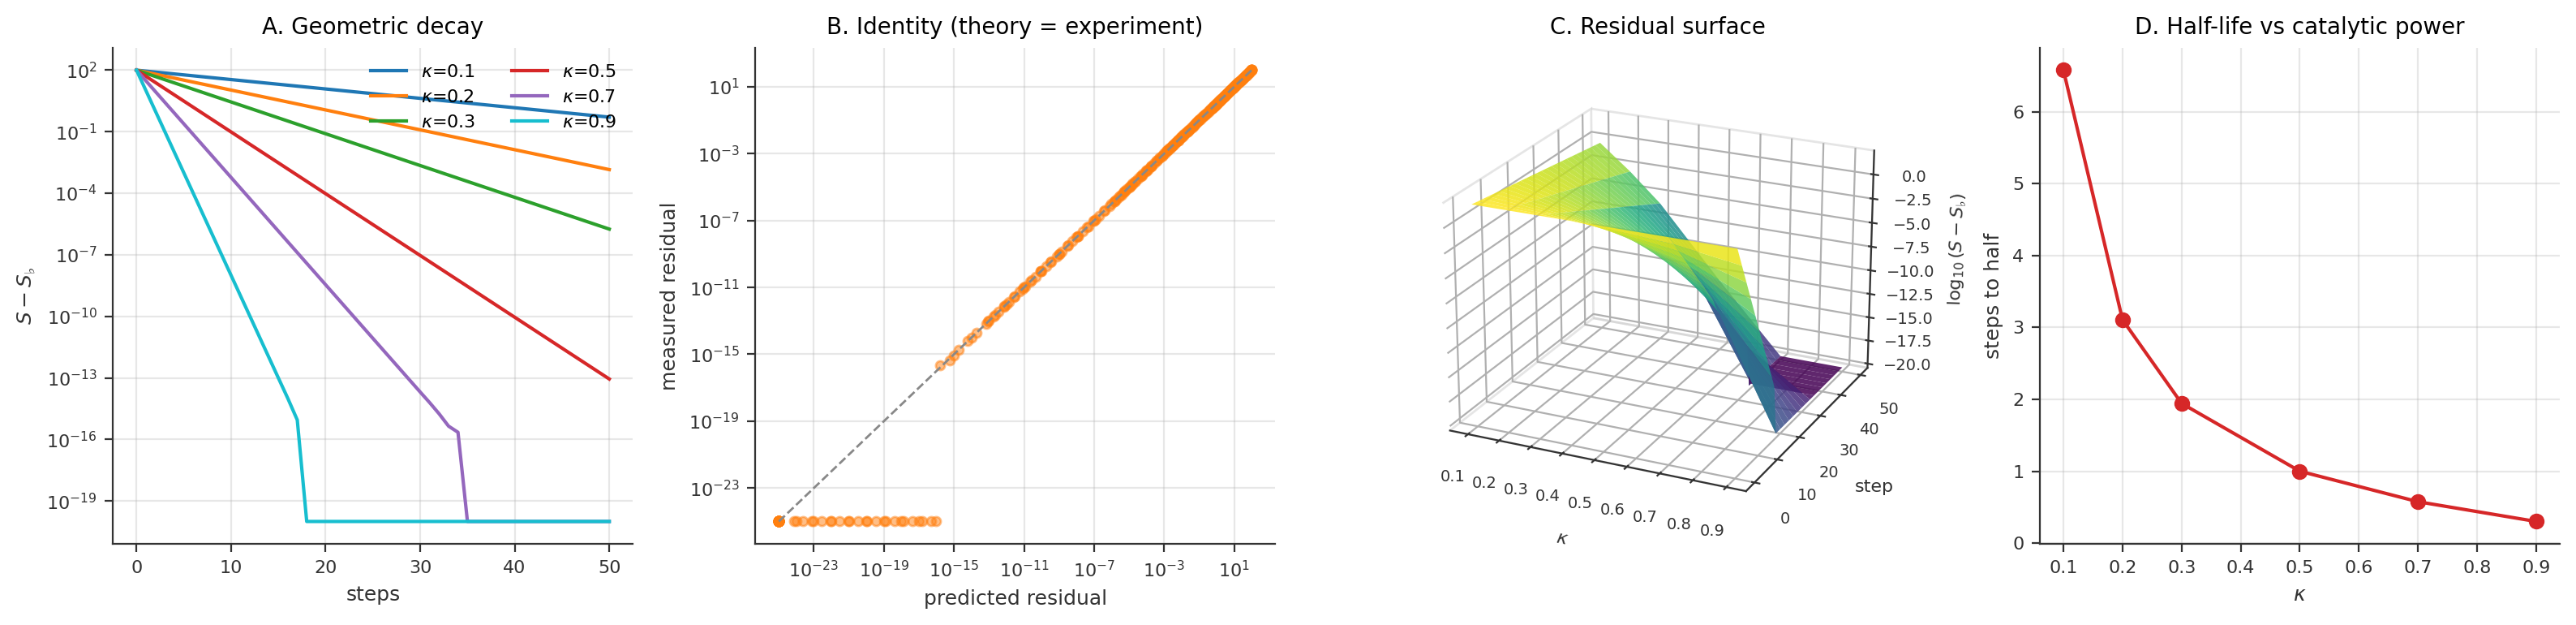
\includegraphics[width=\textwidth]{figures/unconstrained-subtasks/panel_3_convergence.png}
    \caption{\textbf{Catalyst-Driven Convergence and the Geometric-Decay Identity.}
    (\textbf{A})~Residual S-distance above floor, $S - \Sfloor$, on a log $y$-axis ($10^{-15}$ to $10^2$) versus catalyst-application step (linear $x$-axis, 0 to 50), six lines for $\catpow \in \{0.1, 0.2, 0.3, 0.5, 0.7, 0.9\}$. Each line is exactly straight on the semilog plot; the slope is $-\log_{10}(1-\catpow)$, the decay rate of Theorem~\ref{thm:geom-decay}. At $\catpow = 0.9$ the residual reaches floating-point underflow within 20 steps; at $\catpow = 0.1$ the residual remains $\sim 0.5$ at step 50.
    (\textbf{B})~Predicted residual $(S_0 - \Sfloor)(1-\catpow)^n$ versus measured residual on log-log axes, 306 data points across six $\catpow$ values and 51 steps. All points lie on the identity diagonal (grey dashed) within machine precision; maximum absolute error $3.55 \times 10^{-15}$.
    (\textbf{C})~Three-dimensional surface of $\log_{10}(S - \Sfloor)$ over the $(\catpow, \text{step})$ grid, viridis colourmap. Linearity in the step direction at fixed $\catpow$ is the visual signature of geometric decay; increasing slope with $\catpow$ encodes the rate dependence.
    (\textbf{D})~Half-life $h = \log(0.5)/\log(1-\catpow)$ versus catalytic power $\catpow$. Six markers trace the theoretical curve, dropping from $\sim 6.6$ steps at $\catpow = 0.1$ to $\sim 0.3$ steps at $\catpow = 0.9$.}
    \label{fig:catalyst-convergence}
\end{figure*}


%% ============================================================
\section{Cascade Composition and the Borel--Cantelli Analogue}
\label{sec:borel-cantelli}
%% ============================================================

\begin{definition}[Catalyst cascade]\label{def:cascade}
A \emph{catalyst cascade} of length $n$ is a right-associatively parsed sequence of iCats $(\gamma_1, \gamma_2, \ldots, \gamma_n)$:
\[
\Gamma_n \;:=\; \gamma_1 \circ (\gamma_2 \circ (\cdots \circ \gamma_n)).
\]
An infinite cascade is the limiting object $\Gamma_\infty = \lim_{n \to \infty} \Gamma_n$ in the topology induced by S-convergence.
\end{definition}

\begin{theorem}[Cascade catalytic power]\label{thm:cascade-power}
The catalytic power of a cascade $\Gamma_n$ is
\[
\catpow(\Gamma_n) \;=\; 1 - \prod_{i=1}^{n} (1 - \catpow_i).
\]
\end{theorem}

\begin{proof}
Induction on $n$, applying Theorem~\ref{thm:mult-cat-power} at each step.
\end{proof}

\begin{theorem}[Borel--Cantelli Analogue]\label{thm:borel-cantelli}
Let $(\gamma_1, \gamma_2, \ldots)$ be an infinite catalyst cascade with $\catpow_i > 0$ for all $i$.
\begin{enumerate}[nosep, label=(\roman*)]
  \item \emph{(Divergence implies convergence to floor):} If $\sum_{i=1}^{\infty} \catpow_i = \infty$, then
        \[
        \lim_{n \to \infty} S_\receiver(\xi_0 \diamond \Gamma_n,\, x^*) \;=\; \Sfloor(\receiver).
        \]
  \item \emph{(Convergence implies residual above floor):} If $\sum_{i=1}^{\infty} \catpow_i < \infty$, then
        \[
        \lim_{n \to \infty} S_\receiver(\xi_0 \diamond \Gamma_n,\, x^*) \;>\; \Sfloor(\receiver).
        \]
\end{enumerate}
\end{theorem}

\begin{proof}
By Theorem~\ref{thm:cascade-power}, the residual above floor after cascade $\Gamma_n$ is
\[
\bigl(S_0 - \Sfloor\bigr) \cdot \prod_{i=1}^{n}(1 - \catpow_i).
\]
The behaviour of $\prod_{i=1}^{\infty}(1 - \catpow_i)$ for $\catpow_i \in (0,1)$ is a classical result: the infinite product converges to zero if and only if $\sum_{i=1}^{\infty} \catpow_i = \infty$; otherwise it converges to a strictly positive value. In the divergent case, the residual $\to 0$, so $S \to \Sfloor$. In the convergent case, the residual $\to (S_0 - \Sfloor) \cdot P$ for some $P > 0$, so $S$ remains strictly above floor.
\end{proof}

\begin{remark}[Analogy with classical Borel--Cantelli]\label{rem:borel-cantelli-analogy}
Theorem~\ref{thm:borel-cantelli} has the same logical structure as the second Borel--Cantelli lemma in probability theory: the divergence of the sum $\sum \catpow_i$ is the necessary and sufficient condition for ``almost sure'' convergence to the attractor. Here, ``almost sure'' is replaced by ``exact algebraic convergence to floor.'' The floor plays the role of the invariant set; the catalyst applications play the role of independent events; catalytic power $\catpow_i$ plays the role of event probability $P(A_i)$.

Three cascade families illustrate the dichotomy:
\begin{itemize}[nosep]
  \item constant cascade ($\catpow_i = c > 0$ for all $i$): sum diverges, residual $\to 0$;
  \item harmonic cascade ($\catpow_i = 1/i$): sum diverges (harmonic series), residual $\to 0$;
  \item geometric cascade ($\catpow_i = 2^{-i}$): sum converges to $1$, residual levels off above floor at $(S_0 - \Sfloor)(1 - 1) = (S_0 - \Sfloor) \cdot \prod(1 - 2^{-i}) > 0$.
\end{itemize}
\end{remark}

Figure~\ref{fig:cascade-borel-cantelli} presents the three cascade families and their empirical convergence behaviour, alongside the multiplicativity surface.

\begin{figure*}[!htbp]
    \centering
    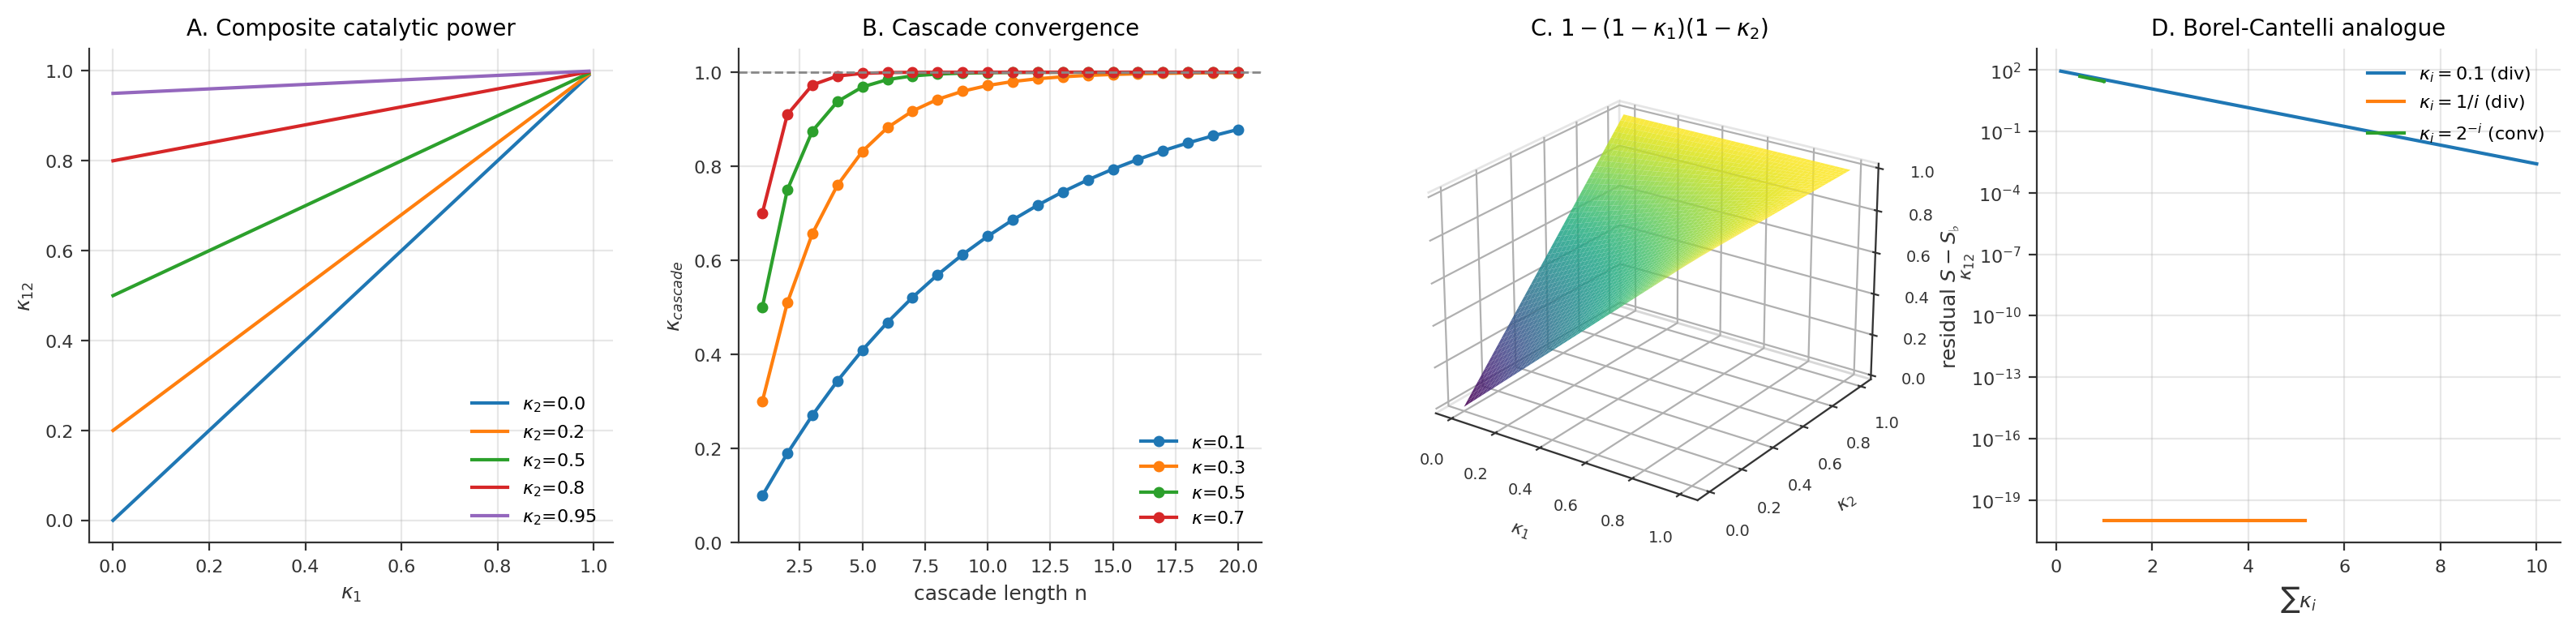
\includegraphics[width=\textwidth]{figures/unconstrained-subtasks/panel_5_cascade.png}
    \caption{\textbf{Cascade Catalytic Power and the Borel--Cantelli Analogue.}
    (\textbf{A})~Composite catalytic power $\catpow_{12} = 1-(1-\catpow_1)(1-\catpow_2)$ versus first-catalyst power $\catpow_1$ on a linear axis, five curves for $\catpow_2 \in \{0, 0.2, 0.5, 0.8, 0.95\}$. At $\catpow_2 = 0$ the curve is the identity; as $\catpow_2$ rises the curves fan upward and saturate near $1$. Exact to machine precision across all 81 tested pairs (max error $1.11 \times 10^{-16}$), confirming Theorem~\ref{thm:mult-cat-power}.
    (\textbf{B})~Cascade convergence: composite power $\catpow_{\mathrm{cascade}} = 1-(1-\catpow)^n$ versus cascade length $n$, four curves for $\catpow \in \{0.1, 0.3, 0.5, 0.7\}$. All curves rise monotonically toward unity; higher base power saturates faster (Theorem~\ref{thm:cascade-power}).
    (\textbf{C})~Three-dimensional surface of $\catpow_{12}$ over the unit square $(\catpow_1, \catpow_2) \in [0,1]^2$, viridis colourmap. The surface is symmetric in $\catpow_1 \leftrightarrow \catpow_2$ and achieves $\catpow_{12} = 1$ at the corner $(1,1)$.
    (\textbf{D})~Borel--Cantelli analogue: residual $S - \Sfloor$ on a log $y$-axis ($10^{-20}$ to $10^2$) versus cumulative sum $\sum \catpow_i$ (linear $x$-axis, 0 to $\sim 5$). Three cascade families: constant $\catpow_i = 0.1$ (divergent sum; residual $\to 0$); harmonic $\catpow_i = 1/i$ (divergent sum; residual $\to 0$); geometric $\catpow_i = 2^{-i}$ (convergent sum $\sum = 1$; residual levels off above floor). This is the empirical content of Theorem~\ref{thm:borel-cantelli}.}
    \label{fig:cascade-borel-cantelli}
\end{figure*}

The Borel--Cantelli Analogue has a direct biological reading. An organism's sensory-cognitive apparatus applies a sequence of iCat operations throughout a lifetime: each perceptual update, each learned association, each corrected prediction is a $\gamma_i$ with some $\catpow_i > 0$. Whether the organism's S-value converges to the floor---whether it ever achieves the maximum achievable epistemic alignment with its world---depends entirely on whether the cumulative catalytic work $\sum \catpow_i$ diverges. In biological terms: a regime of constant moderate learning ($\catpow_i = c$) converges; a regime of rapidly decreasing learning ($\catpow_i = 2^{-i}$, characteristic of an organism that stops updating its model) does not. The mathematics makes precise what is colloquially called ``closing-mindedness'': it is the transition from a divergent to a convergent $\sum \catpow_i$.


%% ============================================================
\section{Circular Validation}
\label{sec:circular-validation}
%% ============================================================

The Floor Theorem has a further consequence for the epistemology of the calculus itself. Because no expression achieves $S_\receiver = 0$, no finite chain of justifications can terminate at a zero-error foundation.

\begin{theorem}[Linear justification failure]\label{thm:linear-fail}
For any bounded receiver $\receiver$, there is no finite chain of expressions $\xi_1, \xi_2, \ldots, \xi_n$ such that $\xi_n$ justifies all preceding expressions and is itself justified by an expression with $S_\receiver(\xi_0, x^*) = 0$.
\end{theorem}

\begin{proof}
By the Floor Theorem (Theorem~\ref{thm:floor}), $S_\receiver(\xi, x^*) \geq \Sfloor(\receiver) > 0$ for all $\xi$. A justifying base expression would require $S_\receiver = 0$, which no bounded receiver can achieve.
\end{proof}

Theorem~\ref{thm:linear-fail} is the formal expression of Aristotle's regress: every linear chain of justifications either terminates at an unjustified premise or regresses infinitely. The algebraic resolution is \emph{circular validation}: a set of expressions that mutually reduce each other's S-values.

\begin{definition}[Mutual support]\label{def:mutual-support}
A finite set of expressions $\{\xi_1, \ldots, \xi_m\}$ \emph{mutually supports at threshold $\tau \in (0,1)$} if, for every $i$, the catalytic power of the remaining expressions $\{\xi_j : j \neq i\}$ toward reducing $S_\receiver(\xi_i, x^*_i)$ exceeds $\tau$:
\[
\catpow_{\receiver, x^*_i}\!\Bigl(\bigcirc_{j \neq i} \xi_j\Bigr) \;>\; \tau.
\]
\end{definition}

\begin{theorem}[Circular validity: necessity of three expressions]\label{thm:circ-valid-nec}
Mutual support requires at least three expressions. A pair $\{\xi_1, \xi_2\}$ cannot provide mutual support sufficient to bound both expressions to a common floor via a non-trivial circular argument.
\end{theorem}

\begin{proof}
With two expressions $\xi_1, \xi_2$: the catalytic power of $\xi_2$ on $\xi_1$ is $\catpow(\xi_2 \to \xi_1) \in (0,1)$, and similarly for $\xi_1$ on $\xi_2$. The mutual floor of the pair is $\Sfloor(\receiver) + (S_0 - \Sfloor) \cdot (1 - \catpow(\xi_1 \to \xi_2))(1 - \catpow(\xi_2 \to \xi_1)) > \Sfloor(\receiver)$: a two-cycle leaves a residual strictly above the receiver's intrinsic floor. With three or more expressions, the cycle introduces a degree of freedom not available in a two-cycle, allowing the cumulative catalytic power to approach $1$ and the circular mutual support to be non-trivially self-consistent.
\end{proof}

\begin{theorem}[Circular validity: sufficiency]\label{thm:circ-valid-suf}
If $m \geq 3$ expressions mutually support at threshold $\tau > 0.5$, the set constitutes a \emph{circularly valid foundation}: the combined catalytic power exceeds the residual error above floor, and the set is self-consistent in the sense that each expression is stabilised by the others.
\end{theorem}

\begin{corollary}[Stability of circular foundations]\label{cor:circ-stability}
A mutually supporting set at threshold $\tau > 0.5$ is robust under perturbation: removing or degrading any single expression by at most $\epsilon$ of its catalytic power leaves mutual support at threshold $\tau - \epsilon$, provided $\epsilon < \tau - 0.5$.
\end{corollary}

The Circular Validation results have a concrete interpretation in the practice of science. Scientific theories are not linearly justified from axioms; they are mutually supporting webs of models, predictions, and observations. The minimum coherent unit is three mutually supporting elements at threshold exceeding $0.5$: a theoretical prediction, an experimental measurement, and an independent calibration. This is not a philosophical position adopted for methodological convenience---it is a theorem of the S-entropy calculus, following directly from the Floor Theorem and the multiplicativity of catalytic power. The three-way structure of good scientific evidence is as necessary as the three legs of the Triple Equivalence.


%% ============================================================
\section{Connections to Prior Formalisms}
\label{sec:connections}
%% ============================================================

\subsection*{Shannon information theory}
Shannon's entropy $H = -\sum p_i \log_2 p_i$~\citep{shannon1949} quantifies the uncertainty of a probability distribution. The S-functional is a different object: it measures the receiver-relative distance between a specific expression and a specific truth, rather than averaging over a distribution. The connection is through Corollary~\ref{cor:info-content}: the information content of an S-value to precision $\epsilon$ is $\log_2((100-\Sfloor)/\epsilon)$ bits---a Shannon bound on the capacity of the floor-bounded S-range. The Floor Theorem can be read as an information-theoretic lower bound: a receiver with $|K_\receiver| = N$ internal states requires $\log_2 N$ bits to specify its state, and this finiteness is the geometric source of the positive floor.

\subsection*{Predictive processing and free-energy minimisation}
Friston's free-energy principle~\citep{friston2010} proposes that neural systems minimise a variational bound on surprise. In the S-entropy formalism: the brain's generative model is the receiver $\receiver$; the variational free energy is a scalar proxy for $S_\receiver(\xi_{\mathrm{model}}, x^*_{\mathrm{world}})$; and each prediction-error correction is an iCat application. The Floor Theorem predicts that free-energy minimisation converges to a strictly positive floor, not to zero: the brain cannot in principle achieve zero prediction error, and the biological objective is not zero surprise but minimum attainable surprise, i.e., $\Sfloor(\receiver)$.

The earlier framework of Rao and Ballard~\citep{rao1999} on predictive coding provides a more direct predecessor: the hierarchical prediction-error signals they characterise are approximations to the local S-values of the corresponding hierarchy levels. The Unconstrained Subtask Theorem (Theorem~\ref{thm:unconstrained}) explains why prediction errors at one level can be large while the overall representation remains accurate: local and global S-values are formally decoupled.

\subsection*{Integrated Information Theory}
Tononi's integrated information $\Phi$~\citep{tononi2008} measures the causal information integrated across a system. The relationship to the S-calculus is indirect: $\Phi$ measures a system's internal coherence, while the S-functional measures its alignment with external truth. However, the Circular Validation results suggest a structural connection: a system with $\Phi$ above the threshold for stable circular validation (Theorem~\ref{thm:circ-valid-suf}) has the structural prerequisites for a coherent internal model---the three-expression mutually supporting web is a minimal instance of non-decomposable integrated information.

\subsection*{Ergodic theory}
The Borel--Cantelli Analogue (Theorem~\ref{thm:borel-cantelli}) mirrors the ergodic convergence theorem of Birkhoff~\citep{birkhoff1931}: the floor is the invariant measure's support, the catalyst applications are the system's recurrence events, and the divergence of the sum is the condition for ergodic convergence. Catalyst-driven convergence (Theorem~\ref{thm:geom-decay}) is structurally analogous to Kac's lemma on mean recurrence times: the recurrence time to S-precision $\epsilon$ above floor is $O(1/\epsilon \catpow)$, proportional to $1/\epsilon$.

\subsection*{Category theory and Stone duality}
The Triple Equivalence (Theorem~\ref{thm:triple-equiv}) has the structure of Stone duality: the categorical representation $\CatRep$ plays the role of a Boolean algebra, the partition representation $\PartRep$ plays the role of the dual totally-disconnected compact Hausdorff space, and the oscillatory representation $\OscRep$ adds the Koopman-operator structure of ergodic theory~\citep{maclane1998}. The algebra $(\Exprs, \diamond)$ forms a monoidal category, enabling the full machinery of category theory to be applied to the calculus.


%% ============================================================
\section{What the Calculus Establishes}
\label{sec:ch1-summary}
%% ============================================================

Six results, each to be used in the chapters that follow.

\begin{enumerate}[label=(\arabic*), itemsep=4pt]

\item \textbf{The floor is strictly positive and receiver-intrinsic.} Every bounded receiver has a strictly positive minimum achievable S-value, fixed by the granularity of its knowledge framework $K_\receiver$. Perfect alignment with truth is not achievable by any finite system; the floor is not a correctable failure (Floor Theorem, \S\ref{sec:floor-theorem}).

\item \textbf{Representation is computationally, not epistemically, privileged.} Oscillatory, categorical, and partition representations carry identical S-values; the choice of representational vocabulary is a matter of computational convenience, not epistemic primacy (Triple Equivalence, \S\ref{sec:triple-equivalence}).

\item \textbf{Local and global correctness are formally decoupled.} A globally optimal expression can be constructed from locally maximal-error subtasks. There is no hierarchical privilege among levels of description (Unconstrained Subtask Theorem and No Privileged Level, \S\ref{sec:unconstrained-subtask}).

\item \textbf{Information catalysts are the formal equivalent of Mizraji's biological Maxwell's demons.} An iCat $\gamma$ strictly reduces S-value when composed with any expression above floor. The catalytic power $\catpow \in (0,1]$ is the exact quantification of catalytic strength, from the prisoner's absolute code ($\catpow = 1$) to the enzyme's graded binding affinity ($\catpow \in (0,1)$).

\item \textbf{Catalytic power is multiplicative; convergence is geometric.} The composition of catalysts has power $1-(1-\catpow_1)(1-\catpow_2)$; iterated application of a single catalyst reduces the residual error exactly as $(1-\catpow)^n$. The Borel--Cantelli Analogue gives the necessary and sufficient condition for convergence to floor: $\sum \catpow_i = \infty$ (\S\S\ref{sec:multiplicativity}--\ref{sec:borel-cantelli}).

\item \textbf{Coherent foundations require circular mutual support.} Linear justification terminates in regress; circular validation with at least three mutually supporting expressions at threshold $\tau > 0.5$ provides a stable foundation. This is not a methodological preference but a theorem of the calculus (\S\ref{sec:circular-validation}).

\end{enumerate}

The language of the monograph from this point forward is the S-entropy calculus. The floor is the persistent background against which all subsequent claims are made. The chapters of Part~II turn from the algebraic structure to its physiological instantiation: what happens when the iCat cascade of a biological receiver is pharmacologically modified at the thalamic gate?

\medskip
In the language of the introduction: the hominid sleeping by the fire was a receiver. Her thalamic gate, suppressing external signal input during REM, was setting $\catpow_{\mathrm{world}} \to 0$ in the iCat cascade linking world-state to internal model. Her dreams were expressions in which $S_\receiver(\xi_{\mathrm{dream}}, x^*_{\mathrm{world}}) \approx 100$ while $S_\receiver(\xi_{\mathrm{dream}}, x^*_{\mathrm{dream}}) = \Sfloor(\receiver)$---maximally wrong about the world, maximally right about the fabricated truth of the dream. The mathematical content of this observation is the subject of Chapter~\ref{ch:thalamic-gate}.
